\chapter{Results}
\label{sec:results}
%In this chapter we expect you to list and explain all the results that you have achieved. Pictures can be useful to explain the results. Think about this chapter as something similar to the demo of the oral presentation. You can also include pictures about use-cases (you can also decide to add use cases to the high level overview chapter).

The Secure Password Manager has born as a simple solution to enhance the user experience when managing passwords. With the constant increasing of cyber-attacks and the continuous spreading of services provided by Internet makes the password management a complex and risky task. It not so rare that who needs to remember a password writes it in a piece of paper stored under the keyboard.\newline\newline
This project is based on multiple challenges that have been solved
\begin{itemize}
	\item All users are able to store passwords in a secure way and retrieve them in an easy manner when needed;
	\item Not only, the application is simple an intuitive while hiding all the security solutions adopted. Moreover, the storing and retrieving process of passwords is fast, in order to not mitigate the user experience during the browser usage;
	\item From the point of view of the security, all these aspects have been combined in order to obtain a profitable solution, exploiting the SECube.
\end{itemize}

Ideally, the user will be able to directly used the system by simply plugging in the SECube via the USB port. The user will be able to buy the device already enclosed into a custom plastic package with the firmware ready and flashed. At the first usage, he will be able to setup the master password that will be used to authenticate a manage the passwords via the Chrome extension. The SECube has been the enable device because, thanks to all its security related feature, allows to create a secure environment in which run the application and store the password.\newline\newline
One non-trivial aspect about this project was the heterogeneity of the Operating System (OS). In fact, the middleware, that is the software that connects to the SECube once connected, has been developed and obfuscated for both Windows and Linux OS. So, independently from the operating system, the user is able to use the Secure Password Manager. Not only, the connection the SECube device is based on a secure channel in which the authentication is based on challenges from both parties. From the point of view of the storage usage, no sensible information have been stored there and the session is encrypted on the fly with an RSA 2048 to increase the security. 


In order to avoid the reverse engineering of the code of the Middleware code, the compiled executable has been obfuscated. This mitigate possible attacks that aim to directly reverse engineering the code by de-compiling the application.


Not only this, but the Middleware provides RestFul APIs to the Chrome Extension in a secure manner via HTTPs, using a certificate. For the moment, the certificate is self-signed (refer to Section \ref{sec:know_issues} about Known Issues).\newline\newline
The last component in the chain is the Chrome Extension that, as anticipated before, is able to provide a simplified access and abstract over the complexity of the Secure Password Manager functions via a simple UI. The extension is able to enable the user to:
\begin{itemize}
	\item Login to the extension
	\item Force a logout by blocking the extension
	\item Reading all stored passwords: the list will be available alphabetically only after the authentication but the password field is not visible but default. This is an important feature, because this extension allows to copy the password to the clipboard even without showing it.
	
	This feature, if correctly used, allows to protect against \textit{piggybacking} attacks.
	\item Manage all password: modify and delete
	\item Create a new password record: by default the new record will set the hostname of the website in order to reduce possible user errors
	\item Password generation: one of the most important feature is the generation of random password using a TRNG, which is able to generate true random sequences of bytes that are encoded in the desired characters. Moreover, a character is selected, it must be present in the generated set.
\end{itemize}
One of the most important aspect about the autocomplete functionality is that, it not only increase the usability of the system by automatically setting the username and password of a known site, but allows to disable this feature after a defined amount of time in order to increase the security. This is important because:
\begin{itemize}
	\item Allows the user to re-insert the password each time the Chrome extension is opened; this allows to increase the usability;
	\item Avoid to keep always the extension unlocked for a long period of time, balancing between the security and usability.
\end{itemize}

\subsection{Usecases}
This is a small set of use cases:
\begin{enumerate}
	\item \textbf{Password generation}
	Luca is a student from Politecnico di Torino and due to all online services that he needs to use for his courses, he is using always the same password. He saw his friend Mike very upset because his password was disclosed in the last password breach of a famous Social Network. Luca, that is using the same password for all his accounts, is nervous about the fact that, if disclosed, its password allows to enter not only his Politecnico Portal but also his Online Payment service.\newline
	For this reason, he has installed the Secure Password Manager and one by one, has updated the passwords with new ones generated via the function available on the Chrome extension. Not only, due to the complexity, he has stored them directly into the application and enabled the autocomplete feature to even not worry about to search them.
	\begin{figure}[H]
		\centering
		\begin{subfigure}{.5\textwidth}
			\centering
			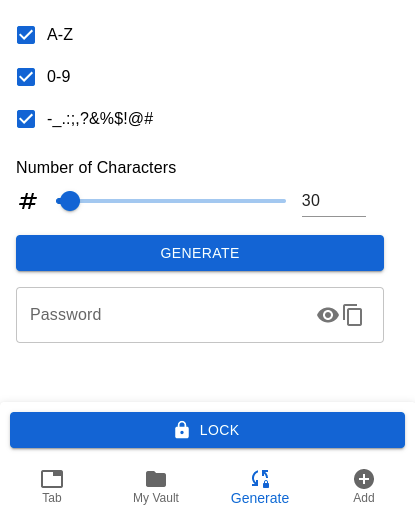
\includegraphics[width=.6\linewidth]{images/extension/generate.png}
			\caption{Random generation of a new password}
			\label{fig:sub1}
		\end{subfigure}%
		\begin{subfigure}{.5\textwidth}
			\centering
			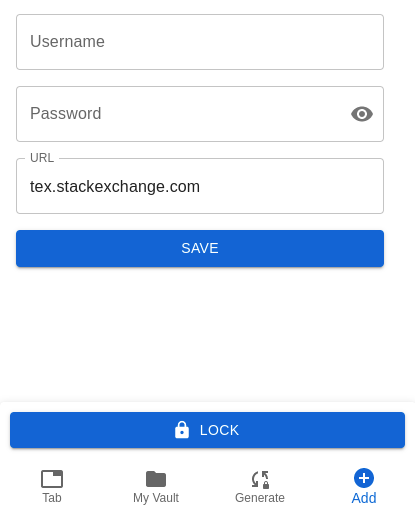
\includegraphics[width=.6\linewidth]{images/extension/add.png}
			\caption{Add of the new password}
			\label{fig:sub2}
		\end{subfigure}
		\caption{Main functions used by Luca}
		\label{fig:test}
	\end{figure}

	\item \textbf{Passwords on multiple computers} Maria is working in an facility in which she has to enter multiple times a day some website to configure and check the connection state of the installed machines. The number of computers is around 10 and the passwords that are used for login into the different websites are very complex. In order to solve this situation, she stored the needed accounts into the Secure Password Manager and, via a distributed command from the central IT department she installed the Secure Password Manager middleware and the chrome extension on all computers. Unfortunately Maria must use directly the computer and can not connect via a remote desktop. In this way, once she arrives in front of the computer and she want to check the machine status via the web page, does not need to enter and remember all the complex passwords she needs. It is enough to remember only the master one of the Secure Password Manager and all other passwords are accessible without the need to store in each one of 10 computers. This increases the security because passwords are never stored in the used computer but stay only into the device.
		\begin{figure}[H]
		\centering
		\begin{subfigure}{.5\textwidth}
			\centering
			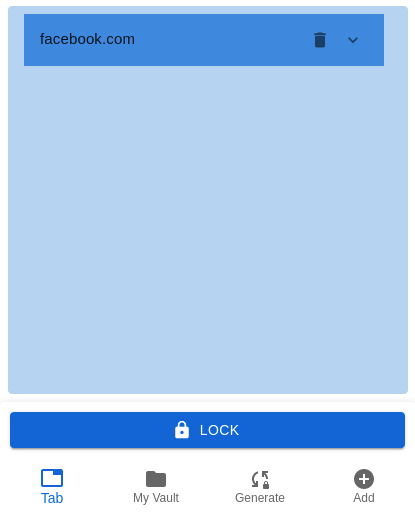
\includegraphics[width=.6\linewidth]{images/extension/popup-lock-tab.png}
			\caption{Access to the current password}
			\label{fig:sub21}
		\end{subfigure}%
		\begin{subfigure}{.5\textwidth}
			\centering
			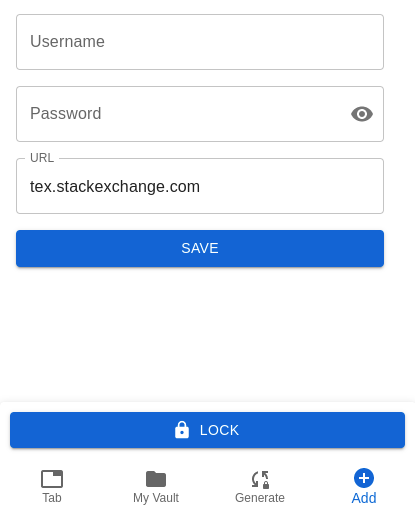
\includegraphics[width=.6\linewidth]{images/extension/add.png}
			\caption{Add of the new password}
			\label{fig:sub22}
		\end{subfigure}
		\caption{Main functions used by Maria}
		\label{fig:tes2t}
	\end{figure}
\end{enumerate}


\section{Known Issues}
\label{sec:know_issues}

\subsection{Host Middleware}
The current certificate has been self signed. In a complete implementation, the certificate must be correctly signed by a certification authority in order to increase the security, that allows the user to not manually accept the certificate the first time the Host Middleware is run.


\subsection{Extension}
\label{sec:extension}
A possible flaw of the extension is the use of the local storage. In fact, as stated by Google
\begin{quote}
    \textit{    Confidential user information should not be stored! The storage area isn't encrypted.
    }
\end{quote}
This may cause some problems regarding privacy. However, to avoid explicit flaws, only the extension options are store in local storage. No sensible information are stored.
\section{Future Work}
\label{sec:future_work}


\subsection{SECube Firmware}
The random password generation is based on the direct mapping from the output of the True Random Noise Generator to the selected characters sets. One option to increase the usability of this project could be to generate password that are easier to be remembered, like concatenating normal words, symbols and number (if selected). This is not a trivial function since, some people could be not familiar with the selected dictionary; the simplest solution is to use words or parts of words that are from the English vocabulary.


\subsection{Host Middleware}
Since now the Middleware application is available for both Windows and Linux. One possible future work is related to the porting to the computer proprietary Operating Systems of Apple (macOS). Being the system completely different, it is based on Unix, which can mitigate the complexity of the porting. The feasibility evaluation of this process is still missing.

\subsection{Extension}
\subsubsection{Local Storage}
Starting from what is explained in \autoref{sec:extension}, a possible improvement is to use a secure storage. For example these data can be encrypted and saved in a secure place. However, this won't allow any kind of synchronization between Google devices, since the local storage can be extended to sync storage, in which data are synced in a place accessible by all chrome devices connected to the same Google account.

\subsubsection{Autocomplete}
The autocomplete feature is working properly on some websites but not on others. In fact, since all web pages are different, the used algorithm is not suitable for all websites. A possible improvement is to use a more general algorithm, which is able to handle all websites.

\subsubsection{Adding and Modifying Notification}
Popular password manager, such as Bitwarden, have two amazing features called \textbf{Login Notification} and \textbf{Change Password Notification}. These features are very useful for the user to automatically track password changes or new accounts.
A possible future work would be to add a notification to ask the user if the username and the password of the new account needs to be saved. By doing this, the user does not have to manually add the new account to My Vault.
The same idea can be applied to the change of password. If the user change the password of an account, the extension can automatically ask the user if the password needs to be updated.

